\documentclass{sig-alternate} 
\usepackage{mathptmx} % This is Times font
\newcommand{\ignore}[1]{}
\usepackage{fancyhdr}
\usepackage[normalem]{ulem}
\usepackage[hyphens]{url}
\setlength{\emergencystretch}{10pt}
\usepackage{graphicx}
\usepackage{multirow}
\usepackage{breakurl}
\usepackage{tabularx}
\usepackage{balance}
\usepackage[nocompress]{cite}
\usepackage{subfig}
\usepackage{hyphenat}
\usepackage{xcolor}
\usepackage{soul}
\usepackage{dcolumn}
\newcolumntype{d}{D{.}{.}{2.1}}
\usepackage{pifont}
%\usepackage{flushend}
\usepackage{booktabs}
\usepackage{tikz}
\usepackage{siunitx}
\newcommand*\mycirc[1]{{\large \ding{\numexpr201+#1\relax}}}
% Always include hyperref last
% \usepackage[bookmarks=true,breaklinks=true,letterpaper=true,colorlinks,linkcolor=black,citecolor=blue,urlcolor=black]{hyperref}
% required to break long URLS sanely
% \PassOptionsToPackage{hyphens}{url} \usepackage{hyperref}
\expandafter\def\expandafter\UrlBreaks\expandafter{\UrlBreaks% save the current one 
\do\a\do\b\do\c\do\d\do\e\do\f\do\g\do\h\do\i\do\j% 
\do\k\do\l\do\m\do\n\do\o\do\p\do\q\do\r\do\s\do\t% 
\do\u\do\v\do\w\do\x\do\y\do\z\do\A\do\B\do\C\do\D% 
\do\E\do\F\do\G\do\H\do\I\do\J\do\K\do\L\do\M\do\N% 
\do\O\do\P\do\Q\do\R\do\S\do\T\do\U\do\V\do\W\do\X% 
\do\Y\do\Z\do\*\do\-\do\~\do\'\do\"\do\-}%

% Ensure letter paper
\pdfpagewidth=8.5in
\pdfpageheight=11in
\pagenumbering{arabic}

%%%%%%%%%%%---SETME-----%%%%%%%%%%%%%
\newcommand{\microsubmissionnumber}{265}
%%%%%%%%%%%%%%%%%%%%%%%%%%%%%%%%%%%%

\newcommand*\circled[1]{\tikz[baseline=(char.base)]{
  \node[shape=circle,draw,inner sep=1pt] (char) {#1};}}

%\title{NUMA-Aware GPUs for Multi-Socket Designs}
\title{Beyond the Socket: NUMA-Aware GPUs}

\author{
Ugljesa Milic$^{\mp\ddagger}$,
Oreste Villa$^{\dagger}$,
Evgeny Bolotin$^{\dagger}$,
Akhil Arunkumar$^{\dagger\star}$,\\\\
Eiman Ebrahimi$^{\dagger}$,
Aamer Jaleel$^{\dagger}$,
Alex Ramirez$^{\dagger\ast}$,
David Nellans$^{\dagger}$
\\\\
$^{\mp}$Universitat Polit\`ecnica de Catalinya (UPC), $^{\ddagger}$Barcelona Supercomputing Center (BSC), \\
$^{\dagger}$NVIDIA, $^{\star}$Arizona State University, and $^{\ast}$Google\\
}

\begin{document}

\maketitle
\pagestyle{plain}

\textbf{Summary.} Reaching the limits of a single-GPU die size, next-generation GPU compute accelerators will likely embrace multi-socket designs increasing the core count and memory bandwidth. However, maintaining the UMA behavior of a single-GPU in multi-GPU systems without code rewriting stands as a challenge. We investigate multi-socket NUMA GPU designs and show that significant changes are needed to both the GPU interconnect and cache architectures to achieve performance scalability. We show that application phase effects can be exploited allowing GPU sockets to dynamically optimize their individual interconnect and cache policies, minimizing the impact of NUMA effects. Our NUMA-aware GPU\footnote{\textbf{Original version appears in MICRO 2017:} \\ Ugljesa Milic, Oreste Villa, Evgeny Bolotin, Akhil Arunkumar, Eiman Ebrahimi, Aamer Jaleel, Alex Ramirez, David Nellans. "Beyond the Socket: NUMA-Aware GPUs", in proceedings of 2017 IEEE/ACM International Symposium on Microarchitecture (MICRO 2017)} outperforms a single GPU by 1.5$\times$, 2.3$\times$, and 3.2$\times$ while achieving 89\%, 84\%, and 76\% of theoretical application scalability in 2, 4, and 8 sockets designs respectively. Implementable today, NUMA-aware multi-socket GPUs may be a promising candidate for performance scaling of future compute nodes.



\textbf{Motivation and Prior Work.} Over the past 10 years, GPUs have become a significant component in datacenter, high performance computing (HPC), and machine learning installations, improving the performance of many workloads by exploiting available data parallelism. Nevertheless, with GPUs nearing the reticle limits for maximum die size and the transistor density growth rate slowing down~\cite{mooredead2016}, developers 
looking to scale the performance of their single GPU programs are in a 
precarious position. Multi-GPU programming models support explicit programming 
of two or more GPUs~\cite{NVIDIAMPI}, but it is challenging to manage multiple GPUs and requires re-writing of traditional single GPU applications,
slowing their adoption.

At the same time, GPUs are starting to expand beyond the traditional PCIe peripheral interface to enable more efficient interconnection
protocols between both GPUs and CPUs~\cite{AMDINFINITYFABRIC,NVLINK}.
Future high bandwidth GPU to GPU interconnects, possibly using
improved communication protocols, may lead to system designs with closely coupled
groups of GPUs that can efficiently share memory at fine granularity.

\begin{figure}[t]
	\centering
	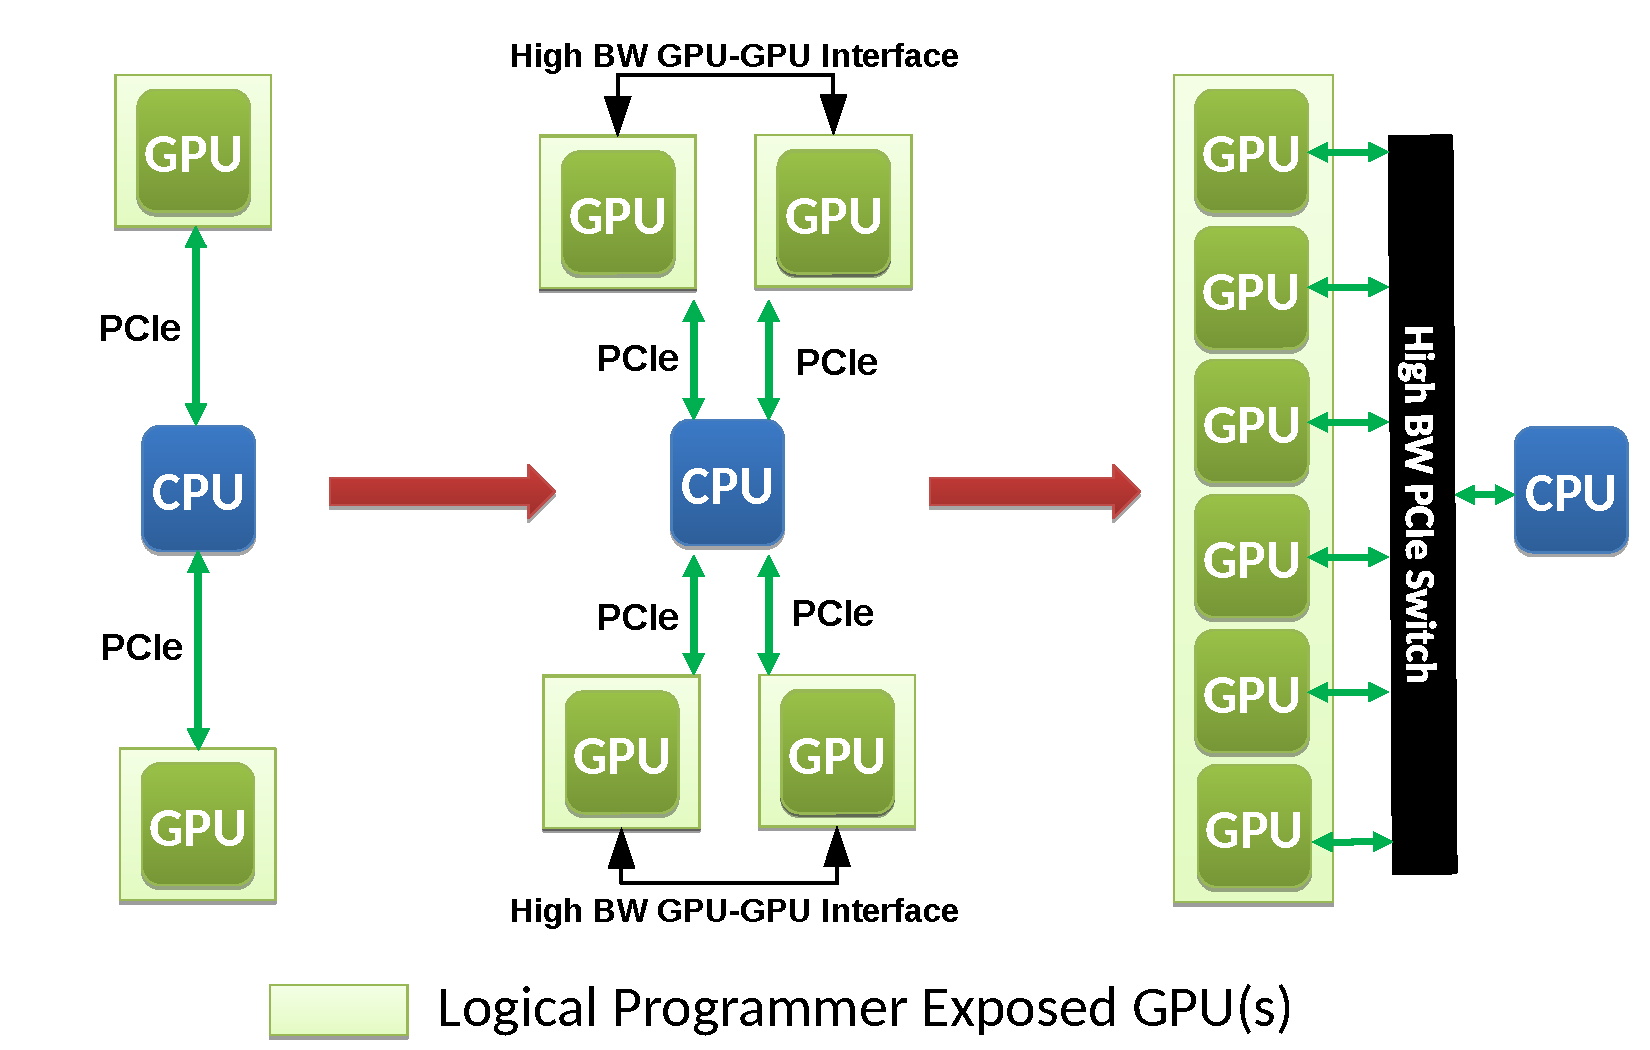
\includegraphics[width=1.0\columnwidth]{figures/inter_gpu_connections.pdf}
	\caption{The evolution of GPUs from traditional discrete PCIe devices to 
		single logical, multi-socketed accelerators utilizing a switched interconnect.}
	\vspace{-0.5cm}
	\label{fig:systemdiagram}
\end{figure}

The onset of such multi-socket GPUs would provide a pivot point for GPU and system vendors. On one hand, vendors can continue to expose these GPUs as 
individual GPUs and force developers to use multiple programming paradigms to 
leverage these multiple GPUs. On the other, vendors could expose multi-socket 
designs as a single non-uniform memory access (NUMA) GPU resource as shown in Figure~\ref{fig:systemdiagram}.  
By extending the single GPU programming model to multi-socket GPUs,  applications 
can scale beyond the bounds of Moore's law, while simultaneously retaining the 
programming interface to which GPU developers have become accustomed.

\begin{figure*}[!t]
	\centering
	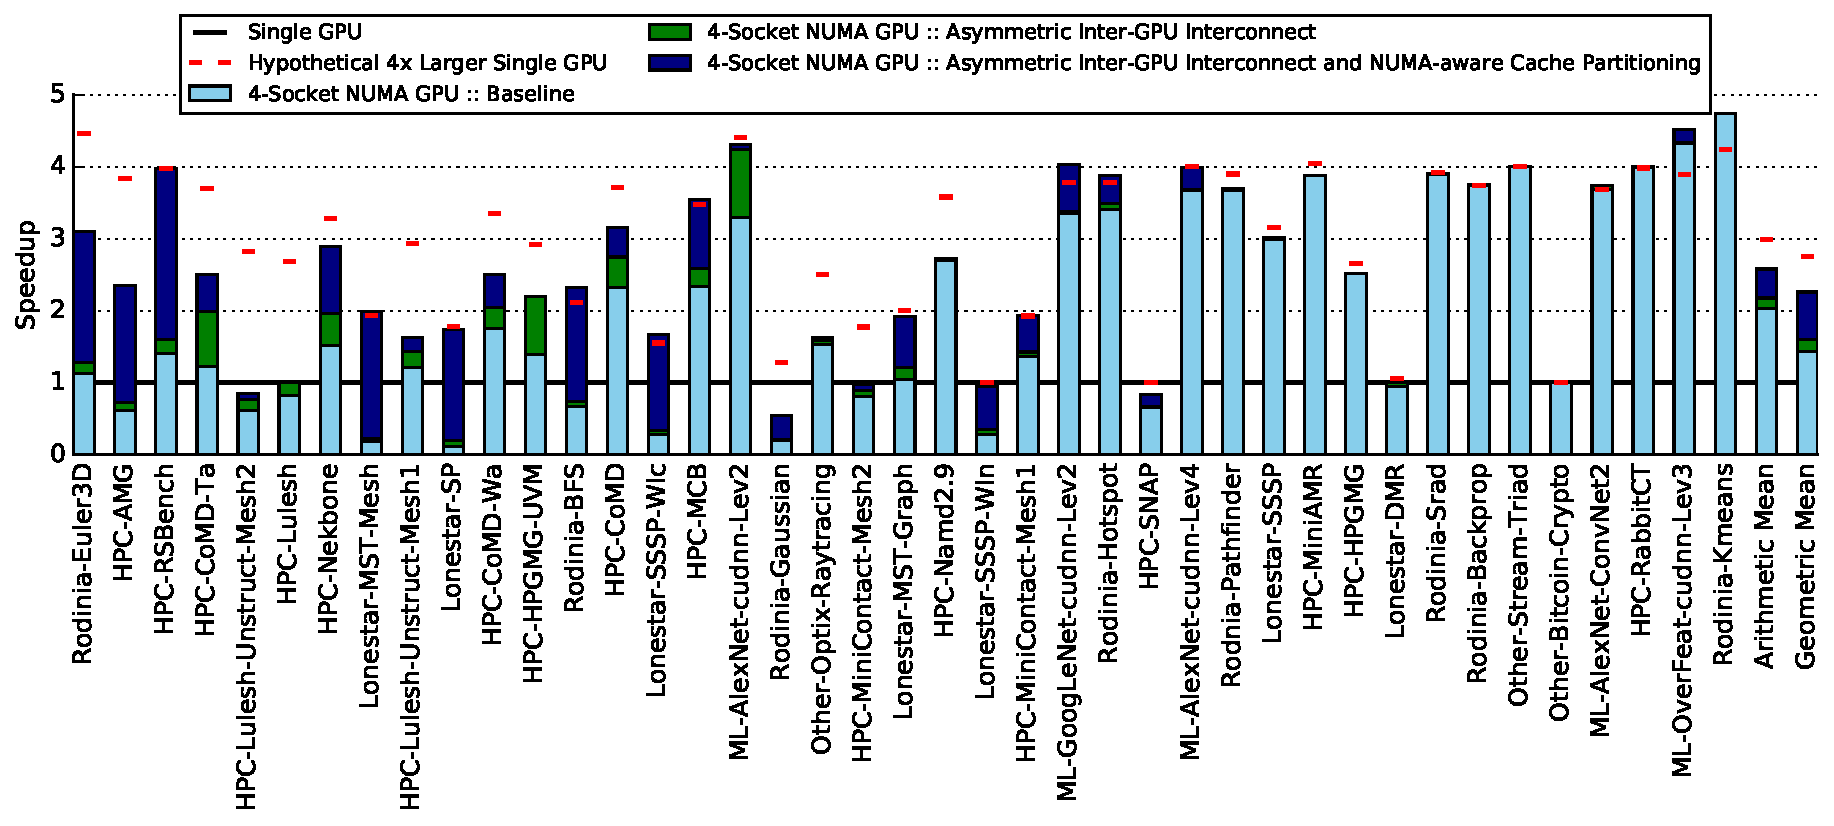
\includegraphics[width=1.0\textwidth]{figures/plot_final_speedup_WB_nvlink_first.pdf}
	\caption{Final NUMA-aware GPU performance compared to a single GPU and 4$\times$ larger single GPU with scaled resources.}
	\label{fig:combined}
\end{figure*}

Several groups have examined aggregating multiple GPUs together under 
a single programming model~\cite{lee2013transparent,Cabezas2015}; however this 
work was done in an era where GPUs had limited memory addressability and relied 
on high latency, low bandwidth CPU-based PCIe interconnects. As a result, prior work focused primarily on improving the multi-GPU programming experience rather than achieving scalable performance. Building upon this work, we propose a 
multi-socket \textit{NUMA-aware} GPU architecture and runtime that aggregates 
multiple GPUs into a single programmer transparent logical GPU. We show that in 
the the era of unified virtual addressing~\cite{UVM}, cache line addressable 
high bandwidth interconnects~\cite{NVLINK}, and dedicated GPU and CPU socket PCB 
designs~\cite{SierraHPC}, scalable multi-GPU performance may be achievable using 
existing single GPU programming models.


\textbf{Asymmetric Interconnect.} In multi-socket NUMA GPU systems, we observe that many applications have different utilization of egress and ingress channels on both a per GPU-socket basis and during different phases of execution. Motivated by these findings, we propose to dynamically control multi-socket link bandwidth assignments, resulting in dynamic asymmetric link capacity on a per-GPU basis. We suggest replacing unidirectional lanes with bi-directional lanes to which we apply an adaptive link bandwidth allocation mechanism that works as following. For each link in the system, at kernel launch the links are always reconfigured to contain symmetric link bandwidth with equal number of lanes per direction. During kernel execution the link load balancer periodically samples the saturation status of each link. If the lanes in one direction are not saturated, while the lanes in the opposite direction are 99\% saturated, the link load balancer reconfigures and reverses the direction of one of the unsaturated lanes after quiescing all packets on that lane. This sample and reconfigure process stops only when directional utilization is not oversubscribed or all but one lane is configured in a single direction.



\textbf{Adaptive Cache Partitioning.} To improve performance in situations where dynamic link balancing is ineffective (both directions saturated), system designers can either increase link bandwidth, which is very expensive, or decrease the amount of traffic that crosses the low bandwidth communication channels. To decrease off-chip memory traffic, architects typically turn to caches
to capture locality.

In NUMA GPUs utilizing traditional memory-side L2 caches is a bad decision. Because memory-side caches only cache accesses that originate in their local memory, they cannot cache memory from other NUMA zones and thus can
not reduce NUMA interconnect traffic. To minimize inter-GPU bandwidth in multi-socket GPU systems we propose processor-side L2 cache and NUMA-aware cache partitioning algorithm applied to both L1 and L2 caches. This cache partitioning policy relies on the same mechanism as adaptive link distribution policy, but this time trying to redistribute cache ways, periodically sampling local and remote memory bandwidth.


\textbf{Final Results. }Figure~\ref{fig:combined} shows the overall improvement NUMA-aware GPUs can achieve when applying both techniques in parallel. Our baseline is a 4-socket locality-optimized GPU with contiguous thread block scheduling and first touch page migration. We observe that on the right side of the graph, some workloads can achieve or surpass the case of a hypothetical 4$\times$ larger monolithic GPU. However, the applications on the left side show a large gap between the baseline NUMA design and theoretical performance. For benchmarks such as \texttt{CoMD}, these features contribute nearly equally to the overall improvement, but for others such as \texttt{ML-AlexNet-cudnn-Lev2} or \texttt{HPC-MST-Mesh1}, interconnect improvements or caching are the primary contributor, respectively. On average, we observe that when combined we see
2.1$\times$ improvement over a single GPU and 80\% over the baseline 4-socket NUMA GPU using memory side L2 caches; best performance is clearly obtained when applying both features in unison.

To understand the scalability of our approach we study the performance of a NUMA-aware multi-socket GPU compared to a single GPU, when scaled across 2, 4, and 8 sockets, respectively. On average a dual-socket NUMA GPU achieves
1.5$\times$ speedup, while 4 sockets and 8 sockets achieve 2.3$\times$ and 3.2$\times$ speedups respectively. Comparing our NUMA-aware GPU implementation to the scaling that applications could achieve on a hypothetical large single GPU, we see that NUMA GPUs can achieve 89\%, 84\%, and 76\% the efficiency of a hypothetical single large GPU in 2, 4, and 8 socket configurations respectively. This high efficiency factor indicates that our design is able to largely
eliminate the NUMA penalty in future multi-socket GPU designs.


\textbf{Potential Impact.} Over the last decade single GPU performance has scaled thanks to a significant growth in per-GPU transistor count and DRAM bandwidth. Unfortunately, transistor density is slowing significantly and integrated circuit manufacturers are not providing roadmaps beyond \SI{7}{nm}. Moreover, GPU die sizes, which have been also slowly but steadily growing generationally, are expected to slow down due to limitations in lithography and manufacturing cost.

We propose GPU manufacturers to re-examine a tried and trued solution from CPU world, multi-socket GPUs, to scaling GPU performance while maintaining the current ratio of floating point operations per second (FLOPS) and DRAM bandwidth. Today, multi-GPU compute nodes are already available: DGX-1 system with 8 GPUs~\cite{dgx}, Summit and Sierra HPC nodes with 6 GPUs~\cite{summit_supercompute}. However, only a certain subset of applications, already parallelized with MPI benefit from an increased number of GPUs. Our transparent multi-GPU execution proposal allows the code of many accelerated workloads to strong-scale on GPUs. In the recent future, we perceive multiple GPU devices to be more tightly coupled, in a form of a multi-socket design. With NUMA-aware optimizations on both microarchitectural and runtime level, multi-socket GPUs will allow to continue scaling performance even when we hit the end of Moore's Law.

The promise of parallel code is scalability. It holds for chip multiprocessors, where parallel applications scale with the number of core per chip, but they also scale to multi-socket nodes. However, that promise does not hold on GPUs, because crossing the chip boundary with memory referencing was not handled, up till recently. Relaying on dynamic page placement into memory at runtime~\cite{UVM} and interconnects with cache line granularity~\cite{NVLINK}, our proposal enables transparent access to remote memory without the need to modify application source code, allowing to scale across the chip boundaries. An accelerated code that runs on a single-GPU today, may achieve the performance of a next-generation GPU (or better) simply by plugging in another GPU next to it. Still, executing UMA-optimized GPU programs on a multi-socket NUMA GPU results in sub-optimal performance. To improve the scalability, we need NUMA-aware transparent multi-GPU execution. The runtime has to provide data locality through memory page placement and thread block scheduling. Our proposals build on top of that, evaluating NUMA-aware microarchitectural aspects such as adaptive inter-socket link assignments and dynamic cache partitioning.

\textbf{I need a sync from your side here... I was thinking to put one paragraph here hitting on alternatives. 3D stacking is not going to be good that's fine, but not sure if we want to mention MCM. Our proposal may scale worse than MCM, because its bandwidth is more constrained (off-chip << on-package), but MCM will be uber-expensive (super-linear, while multi-GPU cost is linear). Do you think we should go there, and basically undermine the MCM proposal or not?}

We believe that entering the filed of transparent multi-socket GPU execution will start a wave of research similar to one initiated by the idea of multi-socket CPU compute nodes. The main concepts still apply, running threads should access their data locally, and this time it is not the discrepancy between local and remote memory access latency, but bandwidth. There are various challenging problems and open questions (thread block scheduling, dynamic page migration and replication, prefetching strategies, making other parts of GPU architecture NUMA-aware, etc.) that can be studied by conjoined research community willing to solve them together.

\bibliographystyle{IEEEtran}
\bibliography{main}
\end{document}
